\documentclass[12pt,a4paper]{article}

%% --- Packages ---
\usepackage[margin=1in]{geometry}
\usepackage{setspace}
\usepackage{graphicx}
\usepackage{amsmath,amssymb}
\usepackage[hidelinks]{hyperref} % Clickable links, but no ugly boxes
\usepackage{enumitem}
\usepackage{booktabs}   % Professional tables
\usepackage{float}
\usepackage{caption}
\usepackage{listings}   % For code
\usepackage{xcolor}     % For colors
\usepackage{tikz}       % For diagrams
\usetikzlibrary{shapes, arrows.meta, positioning, shadows}
\usepackage{siunitx}
\usepackage[utf8]{inputenc}
\usepackage{microtype}  % Improves font spacing and justification
\usepackage{authblk}    % For author affiliation

%% --- Setup ---
\setstretch{1.15}
\hypersetup{
    colorlinks=true,
    linkcolor=blue!60!black,
    citecolor=blue!60!black,
    urlcolor=blue!60!black
}

%% --- Code Listing Style ---
\definecolor{codegreen}{rgb}{0,0.6,0}
\definecolor{codegray}{rgb}{0.5,0.5,0.5}
\definecolor{codepurple}{rgb}{0.58,0,0.82}
\definecolor{backcolour}{rgb}{0.95,0.95,0.92}

\lstdefinestyle{mystyle}{
    backgroundcolor=\color{backcolour},   
    commentstyle=\color{codegreen},
    keywordstyle=\color{magenta},
    numberstyle=\tiny\color{codegray},
    stringstyle=\color{codepurple},
    basicstyle=\ttfamily\footnotesize,
    breakatwhitespace=false,         
    breaklines=true,                 
    captionpos=b,                    
    keepspaces=true,                 
    numbers=left,                    
    numbersep=5pt,                  
    showspaces=false,                
    showstringspaces=false,
    showtabs=false,                  
    tabsize=2
}
\lstset{style=mystyle}

%% --- Title and Authors ---
\title{\textbf{Adaptive Real-Time Stream Analytics using Probabilistic Sketches with Load-Aware Request Routing}\\
\large Phase 1 Detailed Project Report}

\author[1]{Palak Khemchandani}
\author[1]{Naman Aggrawal}
\author[1]{Abhinav Dogra}
\affil[1]{Department of Computer Science, The LNM Institute of Information Technology\\
\vspace{0.5em}
\textbf{Faculty Mentor:} Dr. Subrat K Dash}
\date{\today}

\begin{document}

\maketitle
\thispagestyle{empty}

\begin{abstract}
\noindent Real-time analysis of high-velocity event streams is a cornerstone requirement for modern monitoring, telemetry, and analytics platforms. Exact methods are often infeasible due to memory and latency constraints. This report details the Phase~1 implementation of an adaptive stream analytics architecture that utilizes memory-efficient probabilistic sketches (Count-Min Sketch, HyperLogLog, and Sliding-Window Misra--Gries). In this phase, we have successfully developed the core ingestion pipeline via Kafka, distributed sketch processing workers in both Python and high-performance C++, a shared state store via Redis, and an interactive real-time Web Dashboard with a FastAPI backend. We outline our system architecture, implementation milestones achieved so far, and lay the groundwork for the adaptive controller and load-aware routing optimizations to be completed in subsequent phases.
\end{abstract}

\vspace{1em}
\noindent\textbf{Keywords:} streaming analytics, probabilistic sketches, Count-Min Sketch, HyperLogLog, Misra--Gries, high-velocity data, real-time dashboard.

\newpage
\tableofcontents
\newpage

\section{Introduction}
\label{sec:intro}
High-throughput systems such as online advertising platforms, network telemetry, and social media ingest and process millions of events per second. Extracting aggregated signals—such as item frequencies, distinct counts, and heavy hitters—in real time requires sub-linear memory algorithms and minimal per-event processing.

In Phase~1 of our BTP project, we focused on laying a strong foundation for the streaming analytics platform. Our primary objective was to build a robust and scalable pipeline capable of answering core queries without storing every event. The implemented system consists of:
\begin{enumerate}
    \item A reliable, high-throughput event stream ingestion mechanism.
    \item Memory-efficient probabilistic sketches providing approximate summaries.
    \item Both Python-based and hardware-accelerated C++ analytics workers.
    \item A centralized Redis state store for real-time metrics federation.
    \item A FastAPI-based Analytics API alongside an interactive Web Dashboard.
\end{enumerate}
This report discusses the architectural decisions, the mathematical background of the embedded algorithms, and the exact implementation features completed in this phase.

\section{Background: Probabilistic Sketches}
\label{sec:sketches}

\subsection{Count-Min Sketch (CMS)}
The Count-Min Sketch is a two-dimensional array of counters with $d$ hash functions and width $w$. For an event stream, it answers the frequency query: \textit{"How often did item X appear?"}
For an element $x$, the estimate $\hat{f}(x)$ is the minimum of the $d$ counters at positions $h_i(x)$. The error guarantee is bound such that $\hat{f}(x) \le f(x) + \epsilon N$ with probability $1-\delta$.

\subsection{HyperLogLog (HLL)}
HyperLogLog uses stochastic averaging with $m = 2^p$ registers to estimate distinct cardinality. For an event, the hash value determines the register index and the leftmost 1-bit indicates magnitude. It provides a relative standard error of approximately $1.04 / \sqrt{m}$ while maintaining a memory complexity of only $O(m)$ registers.

\subsection{Sliding-Window Misra--Gries}
Misra--Gries maintains candidate items and their counts to detect frequent items ("heavy hitters"). When a new item arrives, it either increments the count of an existing candidate, takes an empty candidate slot, or decrements all item counts. The implemented sliding-window variant adapts to concept drifts by highlighting recent heavy hitters.

\section{System Architecture and Design}
\label{sec:design}

The system architecture implemented in Phase 1 ensures decoupled stream ingestion, processing, and visualization.

\begin{figure}[H]
    \centering
    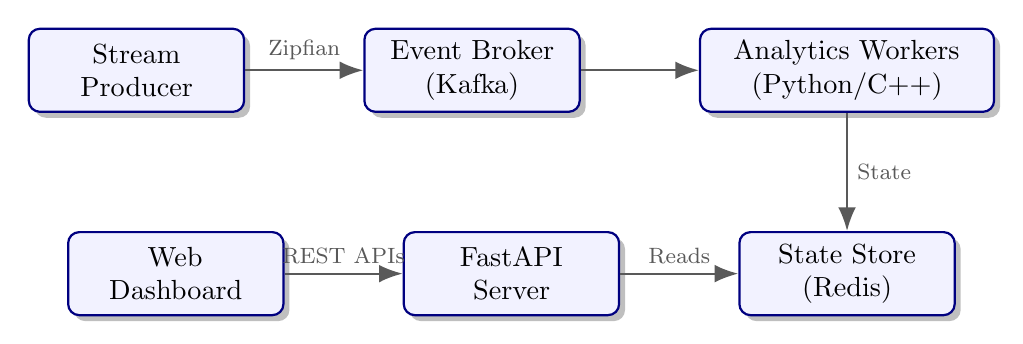
\begin{tikzpicture}[
        node distance=1.5cm,
        auto,
        block/.style={
            rectangle, 
            draw=blue!50!black, 
            fill=blue!5, 
            thick, 
            text width=2.5cm, 
            align=center, 
            rounded corners, 
            minimum height=3em,
            drop shadow
        },
        arrow/.style={
            -{Latex[length=3mm]}, 
            thick, 
            gray!70!black
        }
    ]
        % Nodes
        \node[block] (producer) {Stream\\Producer};
        \node[block, right=of producer] (kafka) {Event Broker\\(Kafka)};
        \node[block, right=of kafka, text width=3.5cm] (workers) {Analytics Workers\\(Python/C++)};
        
        \node[block, below=1.5cm of workers] (state) {State Store\\(Redis)};
        \node[block, left=of state] (api) {FastAPI\\Server};
        \node[block, left=of api] (web) {Web\\Dashboard};

        % Edges
        \draw[arrow] (producer) -- node[midway, above, font=\footnotesize] {Zipfian} (kafka);
        \draw[arrow] (kafka) -- (workers);
        \draw[arrow] (workers) -- node[midway, right, font=\footnotesize] {State} (state);
        \draw[arrow] (api) -- node[midway, above, font=\footnotesize] {Reads} (state);
        \draw[arrow] (web) -- node[midway, above, font=\footnotesize] {REST APIs} (api);
    \end{tikzpicture}
    \caption{Phase 1 system architecture showing data flow from ingestion to visualization.}
    \label{fig:arch}
\end{figure}

\subsection{Stream Ingestion}
We implemented a Stream Producer that generates synthetic events following a Zipfian distribution (heavy-tailed, simulating real web traffic). Events are published to an Apache Kafka topic. We also implemented a Concept Drift simulation that periodically rotates the Zipfian rank distribution.

\subsection{Analytics Workers}
Each worker independently consumes events. We successfully developed workers in two programming environments:
\begin{itemize}
    \item \textbf{Python Worker:} Standard worker computing CMS, HLL, and MG sketches and pushing state telemetry.
    \item \textbf{C++ Worker:} A high-performance drop-in replacement utilizing \texttt{xxHash} (XXH64), \texttt{std::countl\_zero()}, and concurrent read-write locks for lower latency per event. 
\end{itemize}

\subsection{Shared State Store}
Redis plays the role of the shared blackboard. Workers periodically serialize their sketch summaries (like P99 latency, RAM utilization, HLL cardinality, Heavy Hitters) to Redis keys with a TTL constraint.

\section{Phase 1 Implementation Details}
\label{sec:impl}

During this phase, we completed major milestones defining the foundational capability of the system.

\subsection{Web Dashboard Integration}
A fully functional, single-page web dashboard was developed to poll cluster metrics. The dashboard interface includes:
\begin{itemize}
    \item \textbf{Live Sketch Estimates:} Real-time updates of distinct values (HLL) and Top items (CMS + MG).
    \item \textbf{Charts and Latency:} Visualizing P99 latencies and System memory pressure across the worker swarm.
    \item \textbf{Interactive Query Explorer:} An API playground allowing users to evaluate ad-hoc item frequencies natively.
\end{itemize}

\begin{figure}[H]
    \centering
    % Place the screenshot in your Overleaf "images/" directory, e.g., \includegraphics[width=0.9\textwidth]{images/dashboard.png}
    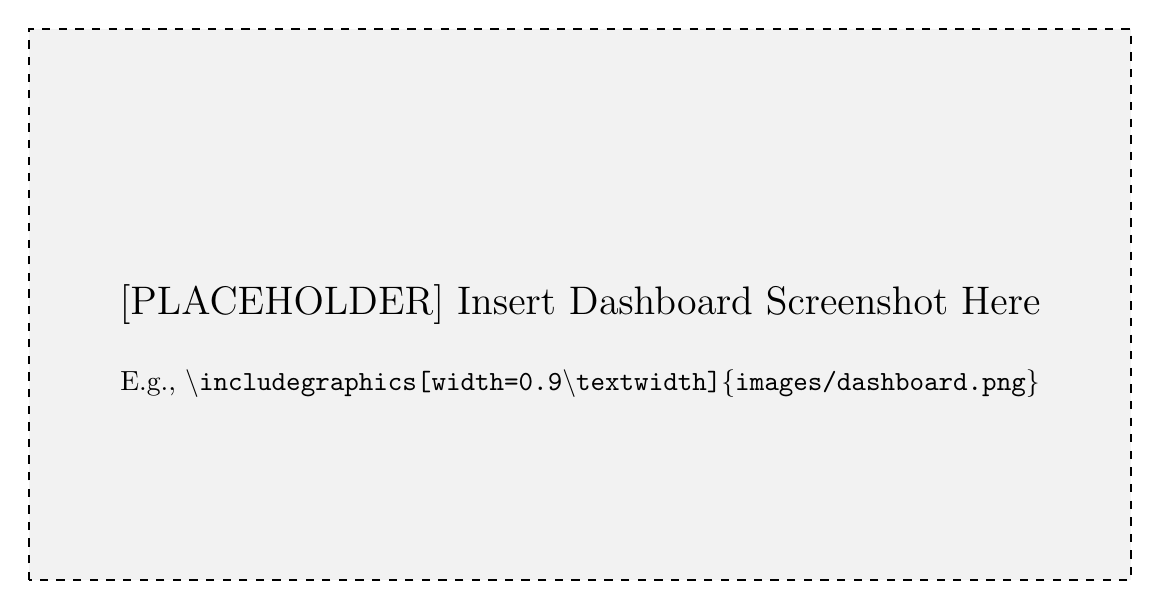
\begin{tikzpicture}
        \draw[thick, dashed, fill=gray!10] (0,0) rectangle (14, 7);
        \node at (7, 3.5) {\Large [PLACEHOLDER] Insert Dashboard Screenshot Here};
        \node at (7, 2.5) {\normalsize E.g., \texttt{\textbackslash includegraphics[width=0.9\textbackslash textwidth]\{images/dashboard.png\}}};
    \end{tikzpicture}
    \caption{Web Dashboard showing live sketch estimates, heavy hitters list, and system latency metrics.}
    \label{fig:dashboard}
\end{figure}

\subsection{System API}
The backend relies on FastAPI handling robust asynchronous requests targeting various analytic endpoints:
\begin{itemize}
    \item \texttt{GET /query/frequency?key=X} \\
    \item \texttt{GET /query/cardinality} \\
    \item \texttt{GET /query/heavy-hitters}
\end{itemize}
These endpoints connect the Web Dashboard directly to the Redis fed sketch telemetry.

\section{Project Plan and Timeline}
\label{sec:plan}

The project is split into foundational (Semester 6) and advanced (Semester 7) components. The current phase establishes everything planned for Phase 1.

\begin{table}[H]
\centering
\renewcommand{\arraystretch}{1.2}
\begin{tabular}{p{0.45\textwidth} p{0.45\textwidth}}
\toprule
\textbf{Semester 6 (Phase 1) - Completed} & \textbf{Semester 7 (Phase 2) - Next} \\
\midrule
Kafka-based stream ingestion (Zipfian) & Dynamic parameter controller \\
Static implementations of CMS, HLL, MG & Load-aware request router implementation \\
High-performance C++ \& Python workers & Robustness testing \& failure injection \\
State management via Redis \& API & Comparative evaluation and Simulations \\
Interactive UI / Real-time Dashboard & Thesis writing and submission \\
\bottomrule
\end{tabular}
\caption{Overall project timeline split by phase, denoting Phase 1 achievements.}
\end{table}

\section{Conclusion}
The first phase of the \textit{Adaptive Real-Time Stream Analytics} project successfully culminated in a distributed, functionally complete stream analytics pipeline capable of ingesting high-throughput streaming events and computing real-time sketches. In upcoming development phases, we will layer dynamic parameter tuning heuristics and advanced load-aware router algorithms to fully accomplish the proposed distributed architecture capabilities.

%% --- References ---
\begin{thebibliography}{9}

\bibitem{cms}
G. Cormode and S. Muthukrishnan. 
\textit{An improved data stream summary: the Count-Min Sketch and its applications.} 
Journal of Algorithms, 2005.

\bibitem{hll}
P. Flajolet, E. Fusy, O. Gandouet, F. Meunier. 
\textit{HyperLogLog: the analysis of a near-optimal cardinality estimation algorithm.} 
AOFA, 2007.

\bibitem{misra}
J. Misra and D. Gries. 
\textit{Finding repeated items.} 
Science of Computer Programming, 1982.

\end{thebibliography}

\end{document}
